\documentclass[xcolor=table]{beamer}
\usetheme{Simple}
\usepackage{tikz}
\usepackage{verbatim}
\usepackage{ulem}
\usetikzlibrary{positioning}
\usepackage{hyperref}
\usepackage{graphicx} 
\usepackage{booktabs} 
\usepackage{mathtools}
\usepackage{listings}
\usepackage{xcolor}

\lstset{
  language=R,
  basicstyle=\ttfamily\tiny,
  commentstyle=\color{blue},
  stringstyle=\color{gray},
  showstringspaces=false,
  breaklines=true,
  frame=single
}

\usepackage[all]{xy}

\title{Graphical Rasch models}
\subtitle{Workshop SAMC 2026, Copenhagen}
\author{Karl Bang Christensen}

\institute{Section of Biostatistics\\Department of Public Health\\University of Copenhagen}

\date{June 11, 2026\\\url{https://biostat.ku.dk/DIGRAM/GRM.pdf}}

\begin{document}

\maketitle

\begin{frame}{Rasch models for measurement}
\begin{block}{Data}
$\boldsymbol{x}=(x_i)_{i=1,\ldots,k}$ is a vector of ordinal responses to $k$ items that all measure the same unidimensional latent variable $\theta$, $\boldsymbol{y}=(y_i)_{i=1,\ldots,m}$ covariates.
\end{block} 
\begin{block}{Structural assumptions}
$$
P(\boldsymbol{x}|\theta,\boldsymbol{y})=\prod_{i=1}^kF_i(x_i,\theta)\;\;\;\;\;\;(LI)\footnote{Assumption/requirement: local independence}
$$
where $F_i(x_i,\theta)$ is independent of the covariates $\boldsymbol{y}$.\footnote{Assumption/requirement: no DIF}
\end{block}
\begin{block}{Parametric assumptions}
\begin{equation}
F_i(x_i,\theta)
=K(\theta,\boldsymbol{\eta}_i)^{-1}\exp(\theta x_i+\eta_{i,x_i})
\label{Rasch}
\end{equation}
\end{block}
\end{frame}

\begin{frame}{4QT\footnote{Staal et al. Geriatr Gerontol Int. 2025;25(2):294-299. doi:10.1111/ggi.15050}}
\begin{center}
\begin{tabular}{
>{\columncolor[HTML]{BBBBBB}}c 
>{\columncolor[HTML]{BBBBBB}}c 
>{\columncolor[HTML]{BBBBBB}}c 
>{\columncolor[HTML]{BBBBBB}}c 
>{\columncolor[HTML]{FFFFFF}}r 
>{\columncolor[HTML]{FFFFFF}}r }
\cellcolor[HTML]{34CDF9}x1 & \cellcolor[HTML]{34CDF9}x2 & \cellcolor[HTML]{34CDF9}x3 & \cellcolor[HTML]{34CDF9}x4 & \cellcolor[HTML]{34CDF9}N & \cellcolor[HTML]{34CDF9}\% \\
0 & 0 & 0 & 0 & 17& 23.61 \\
0 & 0 & 0 & 1 & 2 & 2.78  \\
0 & 0 & 1 & 0 & 3 & 4.17  \\
0 & 1 & 0 & 0 & 4 & 5.56  \\
0 & 1 & 0 & 1 & 5 & 6.94  \\
0 & 1 & 1 & 0 & 4 & 5.56  \\
0 & 1 & 1 & 1 & 1 & 1.39  \\
1 & 0 & 0 & 0 & 4 & 5.56  \\
1 & 0 & 0 & 1 & 1 & 1.39  \\
1 & 0 & 1 & 0 & 1 & 1.39  \\
1 & 1 & 0 & 0 & 7 & 9.72  \\
1 & 1 & 0 & 1 & 8 & 11.11 \\
1 & 1 & 1 & 0 & 9 & 12.50 \\
1 & 1 & 1 & 1 & 6 & 8.33                  
\end{tabular}
\end{center}
% $N=71$ respondents, 1 missing observation.
\end{frame}

\begin{frame}{Instrument validation}
If, in stead of $\boldsymbol{x}=(x_i)_{i=1,\ldots,k}$, we use 
\begin{equation}
\label{score}
R=\sum_{i=1}^kx_i
\end{equation}
do we loose (important) information ?
\begin{block}{Data reduction} 
$\{0,1\}^4\mapsto\{0,1,2,3,4\}$
\end{block}
\end{frame}

\begin{frame}{Rasch model}
Combining (\ref{Rasch}) and (LI)
\begin{equation}
\label{4QT}
P(\boldsymbol{x}|\theta)=K(\theta,\boldsymbol{\eta})^{-1}\exp\left(\theta R+\sum_{i=1}^4\eta_{i,x_i}\right)
\end{equation}
where $R=\sum_{i=1}^4x_i$, i.e. same as (\ref{score}), and $K(\theta,\boldsymbol{\eta})=\prod_{i=1}^4K_i(\theta,\boldsymbol{\eta}_i)$. 

Item parameters $\boldsymbol{\eta}_i=(\eta_{i0},\eta_{i1})=(0,\beta_{i1})$. This means that (\ref{4QT}) can be written
\begin{equation}
\label{also-4QT}
P(\boldsymbol{x}|\theta)=K(\theta,\boldsymbol{\eta})^{-1}\exp\left(\theta R-\sum_{i=1}^4\beta_{i}x_i\right)
\end{equation}
\end{frame}

\begin{frame}{Interpretation of $\beta$'s assuming $E(\theta)=0$}
\begin{center}
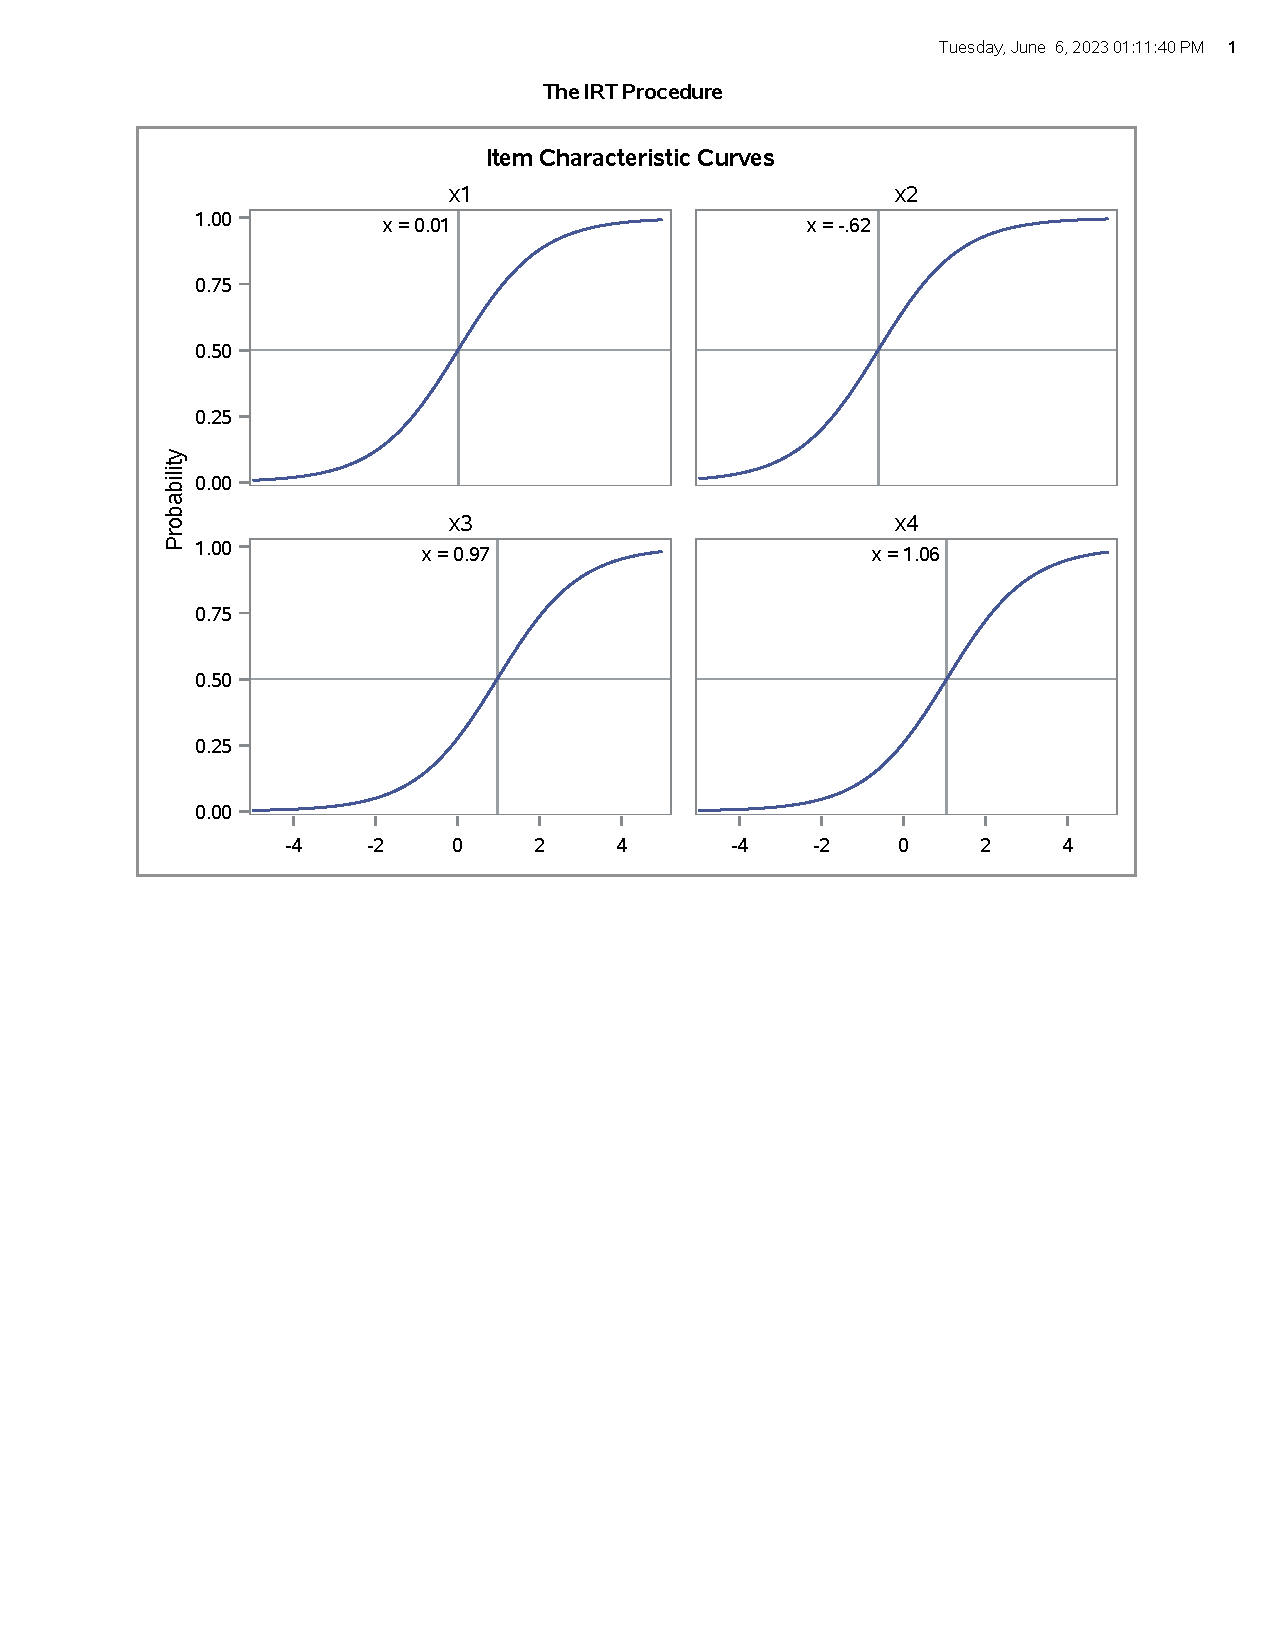
\includegraphics[trim=60pt 370pt 60pt 60pt, clip, scale=0.5]{icc.pdf}
\end{center}
\end{frame}

\begin{frame}{State of the art Rasch analysis}
\lstinputlisting[firstline=10,lastline=18]{4QT.R}
\end{frame}

\begin{frame}{State of the art Rasch analysis}
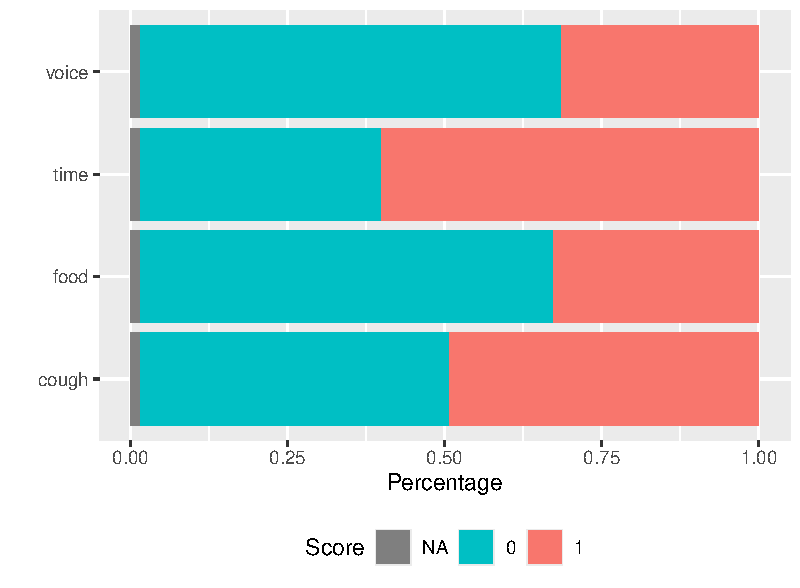
\includegraphics[width=0.8\textwidth]{4QT-items.pdf}
\end{frame}

\begin{frame}{State of the art Rasch analysis}
\lstinputlisting[firstline=21,lastline=22]{4QT.R}
\lstinputlisting[firstline=24,lastline=27]{4QT.R}
Overall model fit is OK (item fit not shown).
\end{frame}

\begin{frame}{Graphical Rasch model}
\lstinputlisting[firstline=29,lastline=40]{4QT.R}
\end{frame}

\begin{frame}{Graphical Rasch model}
\lstinputlisting[firstline=42,lastline=46]{4QT.R}
\end{frame}

\begin{frame}{Graphical Rasch model}
\lstinputlisting[firstline=52,lastline=55]{4QT.R}
\lstinputlisting[firstline=58,lastline=62]{4QT.R}
\end{frame}

\begin{frame}{Local independence (LI)}
\begin{block}{Matters if we look at two respondents ..}
\begin{itemize}
\item .. who are randomly sampled from the population
\item .. who have the same value of $\theta$
\end{itemize}
Low $\theta$: score low on all items. High $\theta$: score high on all items. 
%\pause 
Latent variable $\theta$ is the reason for the correlation. 
%\pause 
The \textbf{only} reason.
\end{block}
\begin{block}{Local independence (LI)}
$$
P(\boldsymbol{x}|\theta)=\underbrace{\prod_{i=1}^k}_{LI}F_i(\theta)
$$
\end{block}
(LI=the absence of LRD).
\end{frame}

\begin{frame}{Origins}


\begin{block}{"The equations of latent structure analysis}
... derive  from the central substantive idea of the whole system, called the principle of local independence, following a suggestion of Mostellor"
\footnotetext{Lazarsfeld, Henry (1968). Boston: Houghton Mifflin. (p.9)}
\end{block}
\pause
\begin{block}{Often cited, but obscure, source}
Andrich (1991).
Book review: Langeheine and Rost ’Latent Trait and Latent
Class Models’.
Psychometrika, 56(1):155–168.    
\end{block}


\end{frame}

\begin{frame}{relatively new to think about LI}
\begin{block}{LI..}
..follows automatically from unidimensionality. It is not an additional assumption\footnotetext{Lord (1980). "Applications of Item Response Theory to Practical Testing Problems". Erlbaum Associates, section 2.4}
\end{block}
\pause
\begin{block}{literature on latent trait models..}
..inclined to define local independence as a special case of unidimensionality\footnotetext{Heinen (1996). "Latent class and discrete latent trait models: Similarities and differences. Thousand Oaks, CA: Sage, p.7}
\end{block}
\end{frame}

\begin{frame}{Overview}
\begin{itemize}
\item[\checkmark] Small data example four dichotomous items. What is validation ?
\item[\checkmark] Local independence (LI). What does it mean ?
\end{itemize}
\begin{block}{Local response dependence (LRD)}
\begin{itemize}
\item[O] consequences
\item[O] analysis
\item[O] interpretation 
\item[O] modelling 
\end{itemize}
\end{block}
\begin{itemize}
\item[O] Data example
\end{itemize}
\end{frame}

\begin{frame}{Evaluate consequences using simulated data}
\begin{block}{Simulate 1000 data sets from}
\begin{itemize}
\item[LI] model (Rasch model without LRD)
\item[LRD] model
\end{itemize}
\end{block}
\begin{block}{Look at consequences for}
\begin{itemize}
\item estimate of reliability
\item item reduction
\end{itemize}
\end{block}
\end{frame}

\begin{frame}{LI and LRD model}
\begin{tabular}{cc}
\xymatrix@=1em{
     &X_1\;&                                                               &Y_1\ar[ddl]                  \\
X_2\;&     &                                                               &                             \\
     &     &\ar@/_/[uul]\ar@/_/[ull]\ar@/^/[dll]\ar@/^/[ddl] \;\;\theta\;\;&                  &Y_2\ar[ll]\\
X_3\;&     &                                                               &Y_3\ar[uuu]\ar[ul]           \\
     &X_4\;&                                                               &
}
&
\xymatrix@=1em{
     &X_1\;&                                                               &Y_1\ar[ddl]                  \\
X_2\;\ar@{-}[ur]&     &                                                               &                             \\
     &     &\ar@/_/[uul]\ar@/_/[ull]\ar@/^/[dll]\ar@/^/[ddl] \;\;\theta\;\;&                  &Y_2\ar[ll]\\
X_3\;&     &                                                               &Y_3\ar[uuu]\ar[ul]           \\
     &X_4\;&                                                               &
}
\end{tabular}
\end{frame}


\begin{frame}{Estimate of reliability}
Compute estimate of reliability and the actual test-retest reliability.
\pause
\begin{block}{LI model}
$\alpha$ is a lower bound for the test-retest reliability
\end{block}
\pause
\begin{block}{LRD model}
$\alpha$ is just a number without any interpretation
\end{block}
Cronbachs coefficient $\alpha$ used here; PSI: same story.
\end{frame}

\begin{frame}{Test-retest correlation}
\begin{center}
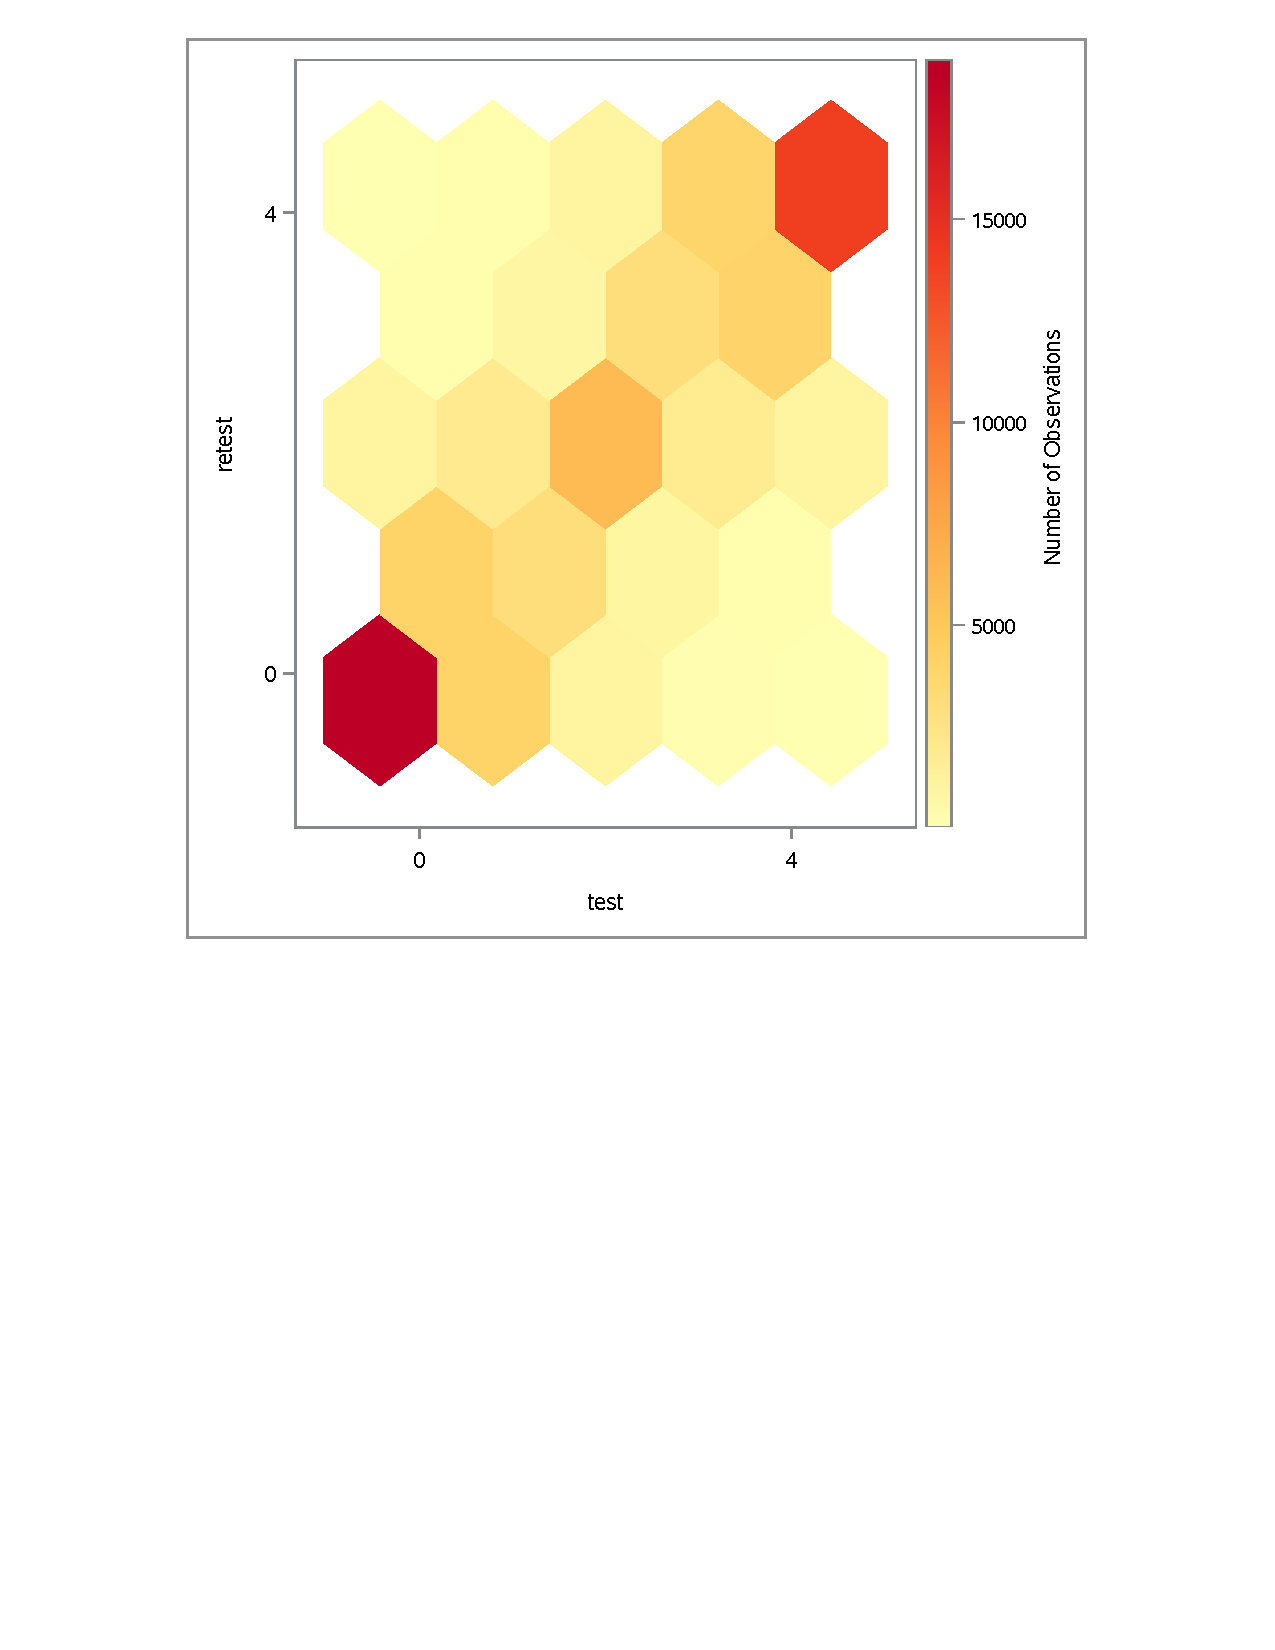
\includegraphics[width=5cm, clip, trim=33mm 122mm 60mm 9mm]{hex1.pdf}
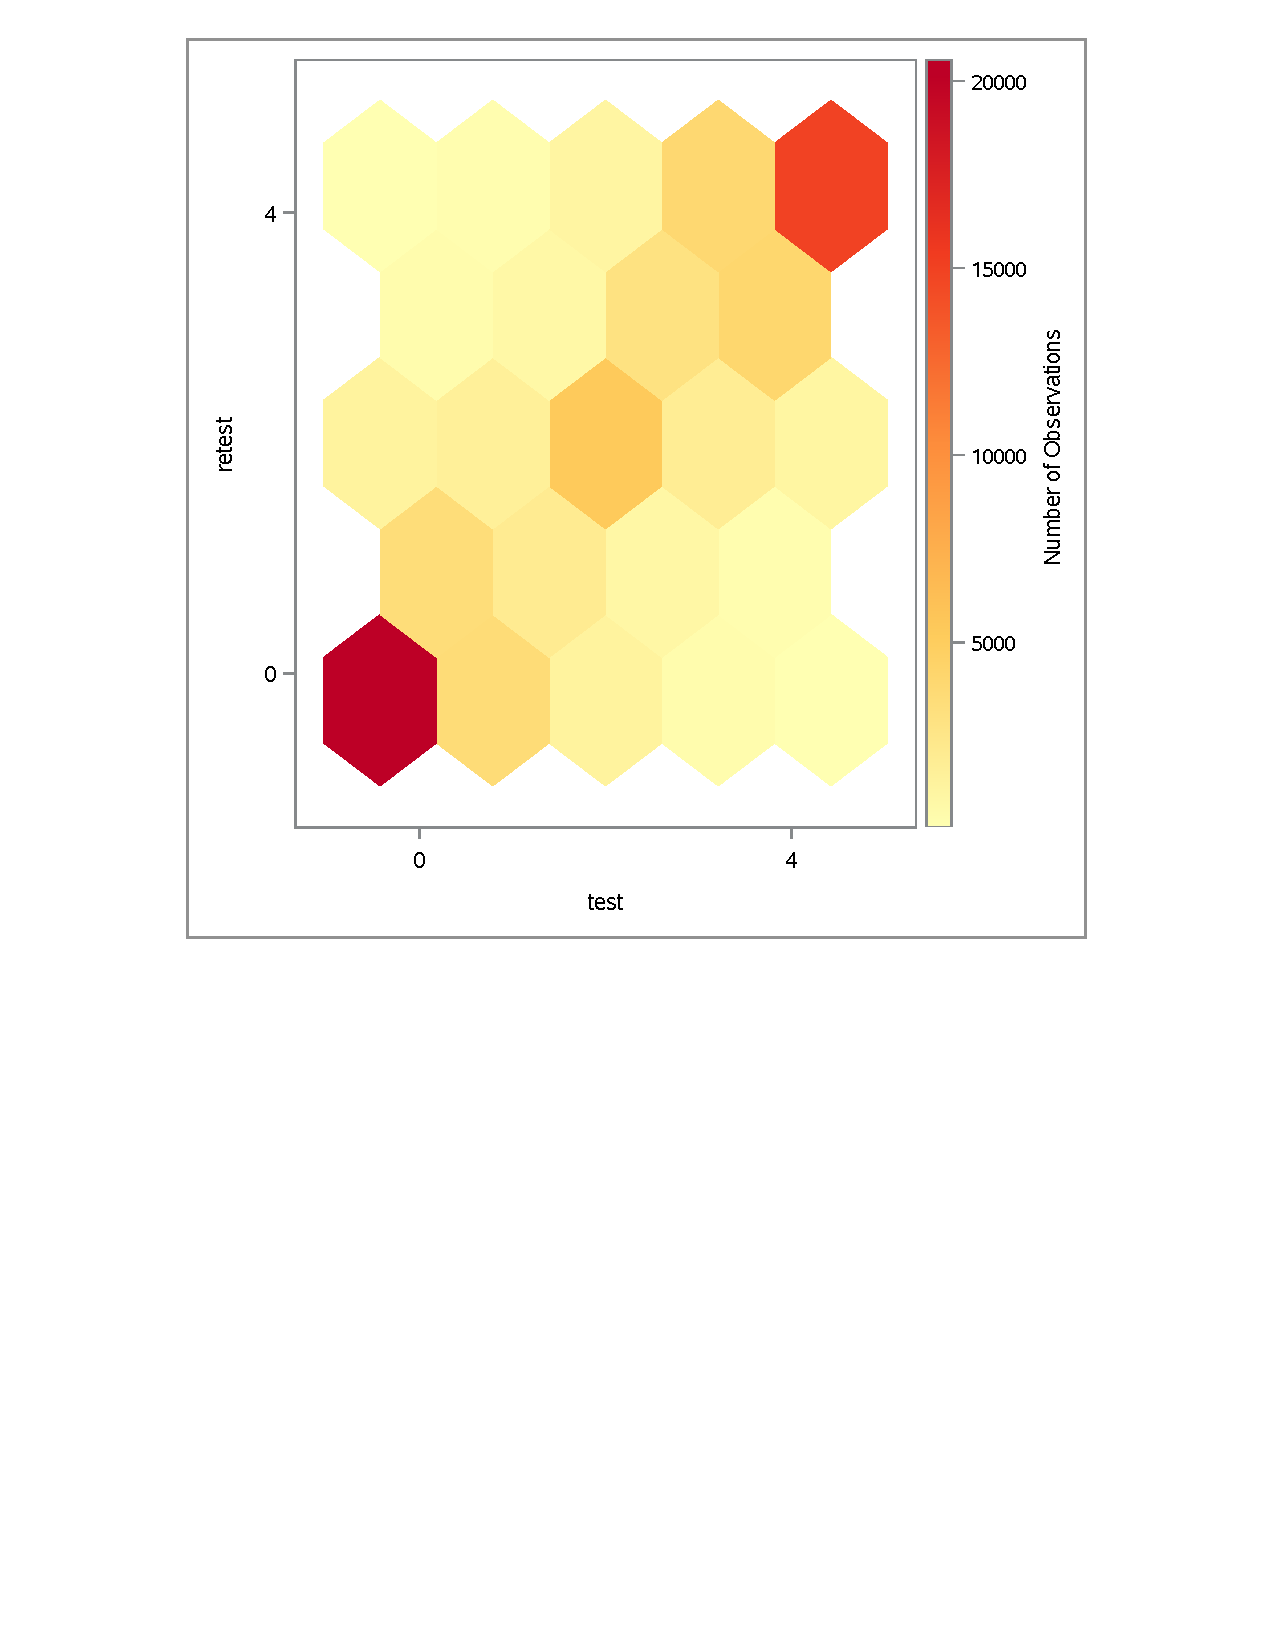
\includegraphics[width=5cm, clip, trim=33mm 122mm 60mm 9mm]{hex2.pdf}
\end{center}
\end{frame}

\begin{frame}{Cronbachs coefficient $\alpha$}
\begin{center}
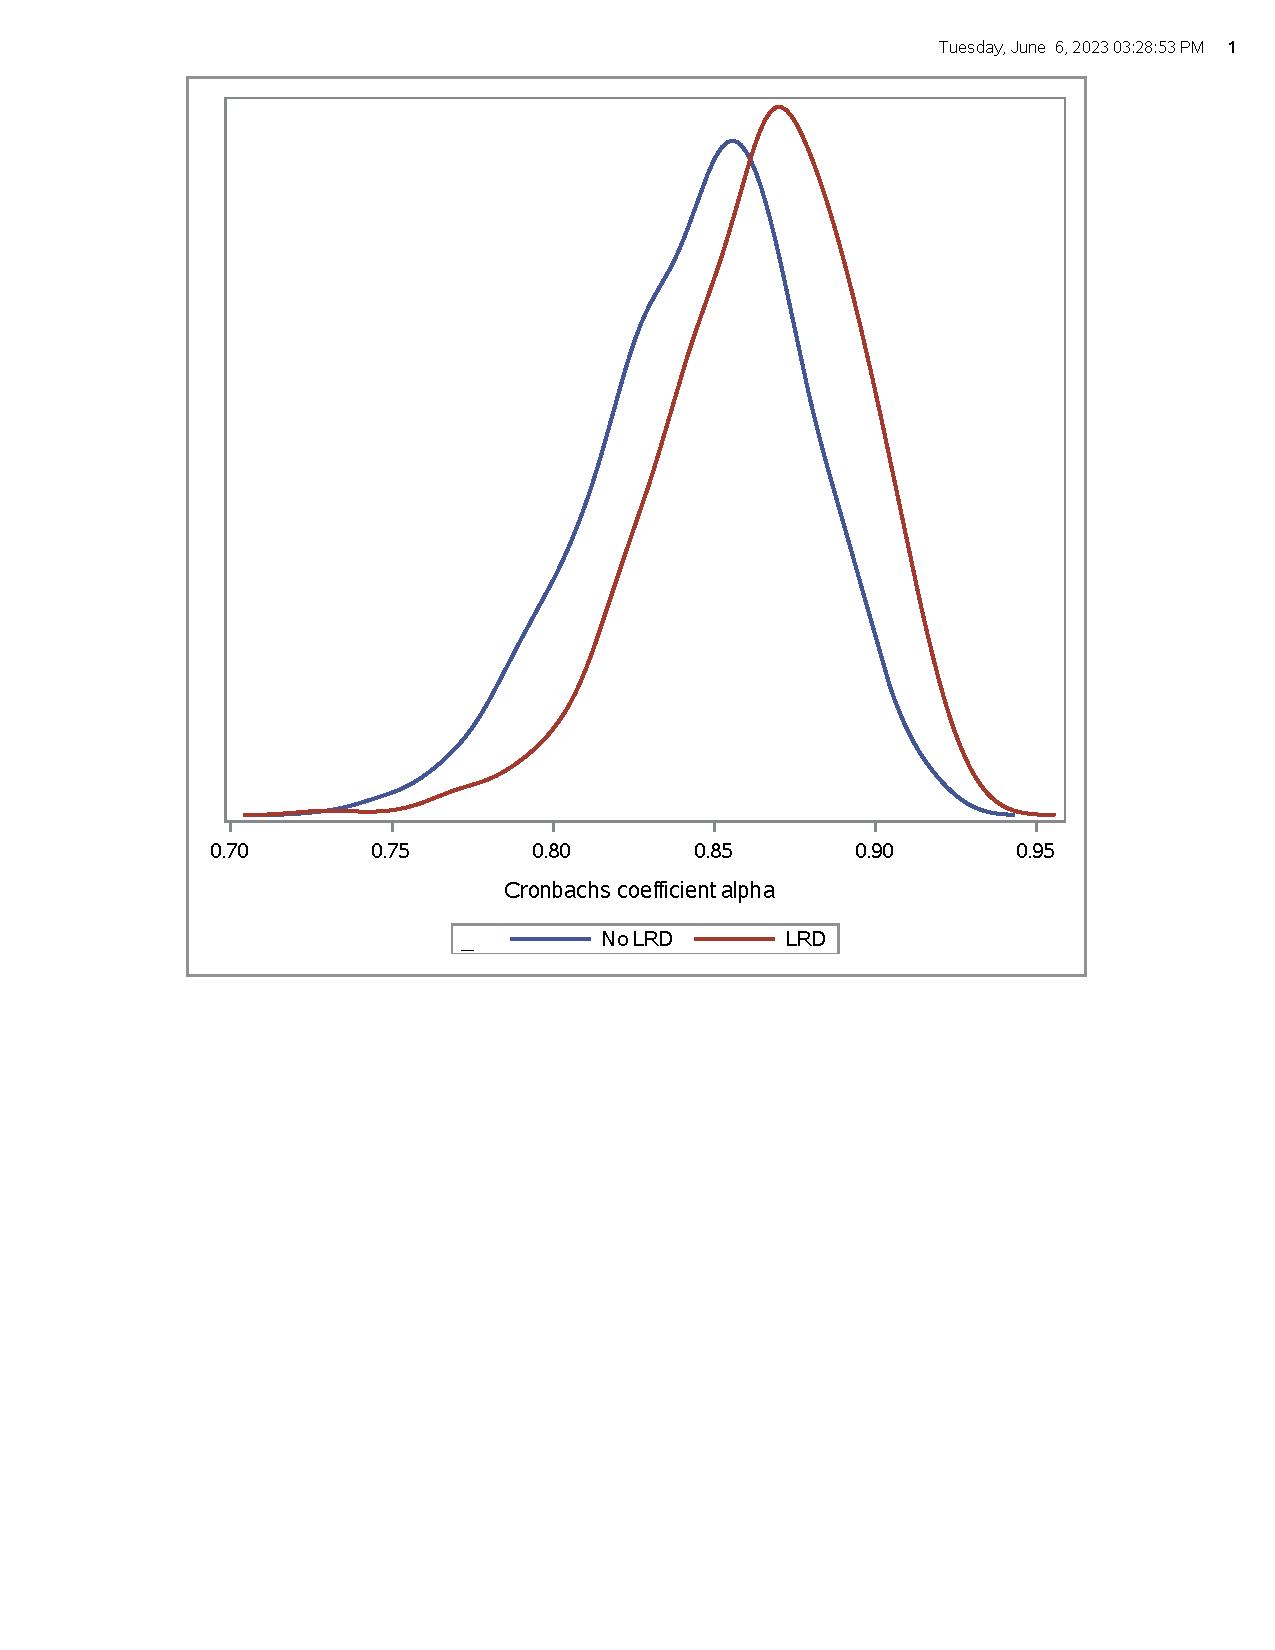
\includegraphics[width=7cm, clip, trim=33mm 124mm 33mm 14mm]{alpha.pdf}
\end{center}
\end{frame}

\begin{frame}{Consequences for item reduction}
How often is an item eliminated ?
\begin{block}{Non-parametric IRT. Item scalability coefficients.}
\begin{tabular}{lrrr}
\hline
Item  & $H_i$ & (95\% CI)      &             \\
\hline
$X_1$ & 0.60  & (0.41 to 0.78) &             \\
$X_2$ & 0.41  & (0.22 to 0.61) &             \\
$X_3$ & 0.24  & (0.02 to 0.45) & \textbf{removed} \\
$X_4$ & 0.25  & (0.03 to 0.46) &            \\
\hline
\end{tabular}
\footnotetext{$H_i$ summarizes Guttman errors}
\end{block}
2PL model: same story
\end{frame}

\begin{frame}{Non-parametric IRT ?? Guttman error ??}
\begin{tabular}{lcccc}
\hline
               & Easy item & middle item & hard item &       \\
\hline
respondent$_1$ & 1         & 0           & 0         &       \\
respondent$_2$ & 1         & 1           & 0         &       \\
respondent$_3$ & 1         & 0           & 1         & \textbf{x} \\
respondent$_4$ & 0         & 1           & 1         & \textbf{x} \\
respondent$_5$ & 1         & 1           & 1         &       \\
:              & :         &             & :         &      \\
\hline
\end{tabular}
\end{frame}

\begin{frame}{Consequences for item reduction}
How often is an item flagged for removal ?
\begin{center}
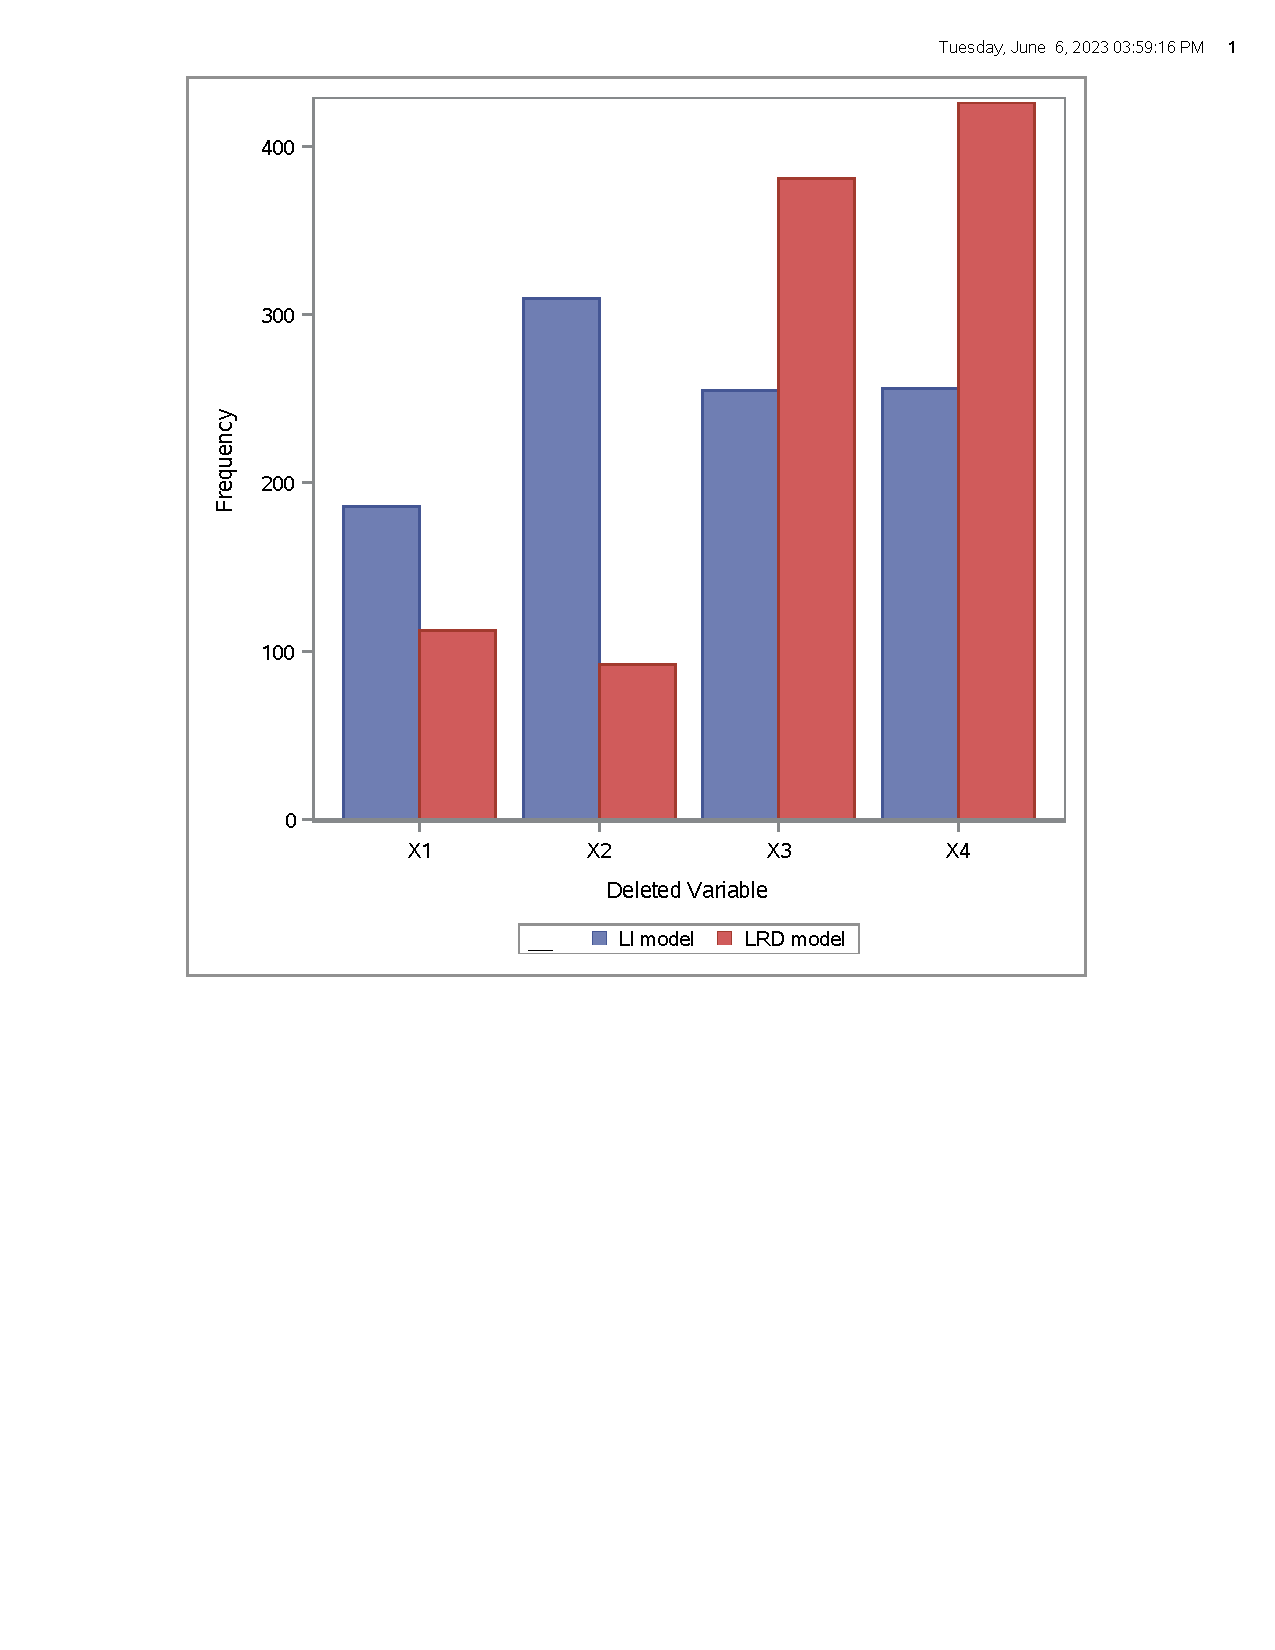
\includegraphics[width=6cm, clip, trim=53mm 115mm 33mm 14mm]{removed.pdf}
\end{center}
\end{frame}

\begin{frame}{Consequences ..}
\pause
\begin{block}{.. estimates of reliability}
Overly optimistic
\end{block}
\pause
\begin{block}{.. for item reduction}
Items with LRD are retained. Bad for content validity.
\end{block}
\end{frame}

\begin{frame}{Overview}
\begin{itemize}
\item[\checkmark] Small data example four dichotomous items. What is validation ?
\item[\checkmark] Local independence (LI). What does it mean ?
\end{itemize}
\begin{block}{Local response dependence (LRD)}
\begin{itemize}
\item[\checkmark] consequences
\item[O] analysis
\item[O] interpretation 
\item[O] modelling 
\end{itemize}
\end{block}
\begin{itemize}
\item[O] Data example
\end{itemize}
\end{frame}

\begin{frame}{Analysis}
\begin{block}{Yens $Q_3$ test statistic}
General IRT approach first suggested by Wendy Yen in 1984. Implemented in RUMM and Winsteps.
\end{block}
\pause
\begin{block}{Item splitting}
Simple approach similar to "splitting for DIF". Easy to do in RUMM or Winsteps.
\end{block}
\pause
\begin{block}{graphical Rasch model}
Extension of the Rasch model that incorporates LRD (and DIF) using log linear interaction parameters
\end{block} 
\end{frame}

\begin{frame}{$Q_3$ test statistic}
\pause
\begin{block}{Estimate}
$(\hat\beta_i)$ and $(\hat\theta_v)$
\end{block}
\pause
\begin{block}{Compute expected data matrix $\boldsymbol{E}=(E_{iv})$} 
$$
E_{iv}=E(X_{iv}|\theta=\hat\theta_v)=\frac{\exp(\hat\beta_i+\hat\theta_v)}{1+\exp(\hat\beta_i+\hat\theta_v)}
$$ 
\end{block}
\pause
\begin{block}{Compute matrix of residuals $\boldsymbol{R}=(R_{iv})$} 
$$
R_{iv}=(X_{iv}-E_{iv})/V(X_{iv})
$$
\end{block}
\pause
\begin{block}{Evaluate} 
correlation between residuals
\end{block}
\end{frame}


\begin{frame}{Yens $Q_3$ test statistic}
Suggested by Yen.\footnote{Yen (1984). Applied Psychological Measurement, 8, 125–145. \url{https://doi.org/10.1177/014662168400800201}} 
\begin{block}{Evaluate} 
correlation between residuals
\pause 
- but how ?
\end{block}
\pause 
Intuitively we expect them to be uncorrelated because the model has explained all the correlation
\pause 
- but is our intuition correct ?
\pause
\begin{block}{Data example} 
$$
\begin{pmatrix*}[r]
 1.000 & -0.332 & -0.309 & -0.360 \\ 
-0.332 &  1.000 & -0.242 & -0.150 \\ 
-0.309 & -0.242 &  1.000 & -0.564 \\ 
-0.360 & -0.150 & -0.564 &  1.000 \\     
\end{pmatrix*}
$$
\end{block}
counter-intuitive at first
\pause
- we are conditioning on the total score.
\end{frame}

\begin{frame}{$Q_{3,\ast}$}
Extensive simulation study indicated that '0.2 above the average' works well in many situations.\footnote{Christensen et al (2017). Applied Psychological Measurement, 41(3), 178–194. \url{https://doi.org/10.1177/0146621616677520}}
\begin{block}{App}
\scriptsize\url{http://publicifsv.sund.ku.dk/~kach/Q3/critical_values_Yens_Q3.html}
\end{block}
summarizes simulation studies. Also addresses the issue of multiple testing.
\end{frame}

\begin{frame}{Item splitting}
Simple idea.\footnote{Andrich, Kreiner (2010). Applied Psychological Measurement, 34, 181-192. \url{https://doi.org/10.1177/0146621609360202}}
Let's pretend that LRD has a direction
$$
\xymatrix@=1em{
     &X_1\;\ar@{->}[dl]&                                                               &Y_1\ar[ddl]                  \\
X_2\;&     &                                                               &                             \\
     &     &\ar@/_/[uul]\ar@/_/[ull]\ar@/^/[dll]\ar@/^/[ddl] \;\;\theta\;\;&                  &Y_2\ar[ll]\\
X_3\;&     &                                                               &Y_3\ar[uuu]\ar[ul]           \\
     &X_4\;&                                                               &
}
$$
\pause
imaginable for, e.g., educational tests. 
\end{frame}

\begin{frame}{Item splitting}
\begin{center}
\begin{tabular}{
>{\columncolor[HTML]{BBBBBB}}c 
>{\columncolor[HTML]{BBBBBB}}c 
>{\columncolor[HTML]{BBBBBB}}c 
>{\columncolor[HTML]{BBBBBB}}c }
\cellcolor[HTML]{34CDF9}x1 & \cellcolor[HTML]{34CDF9}x2$\_$& \cellcolor[HTML]{34CDF9}x2$\_\_$
& \cellcolor[HTML]{34CDF9}x3 \\
0 & 0 &   & 0 \\
0 & 0 &   & 0 \\
0 & 1 &   & 0 \\
0 & 1 &   & 1 \\
0 & 1 &   & 1 \\
1 &   & 0 & 0 \\
1 &   & 0 & 1 \\
1 &   & 1 & 0 \\
1 &   & 1 & 1 \\
1 &   & 1 & 1                   
\end{tabular}
\end{center}
Estimate parameters $\beta_{2\_}$ and $\beta_{2\_\_}$
\end{frame}

\begin{frame}{ICC for extended model}
\begin{center}
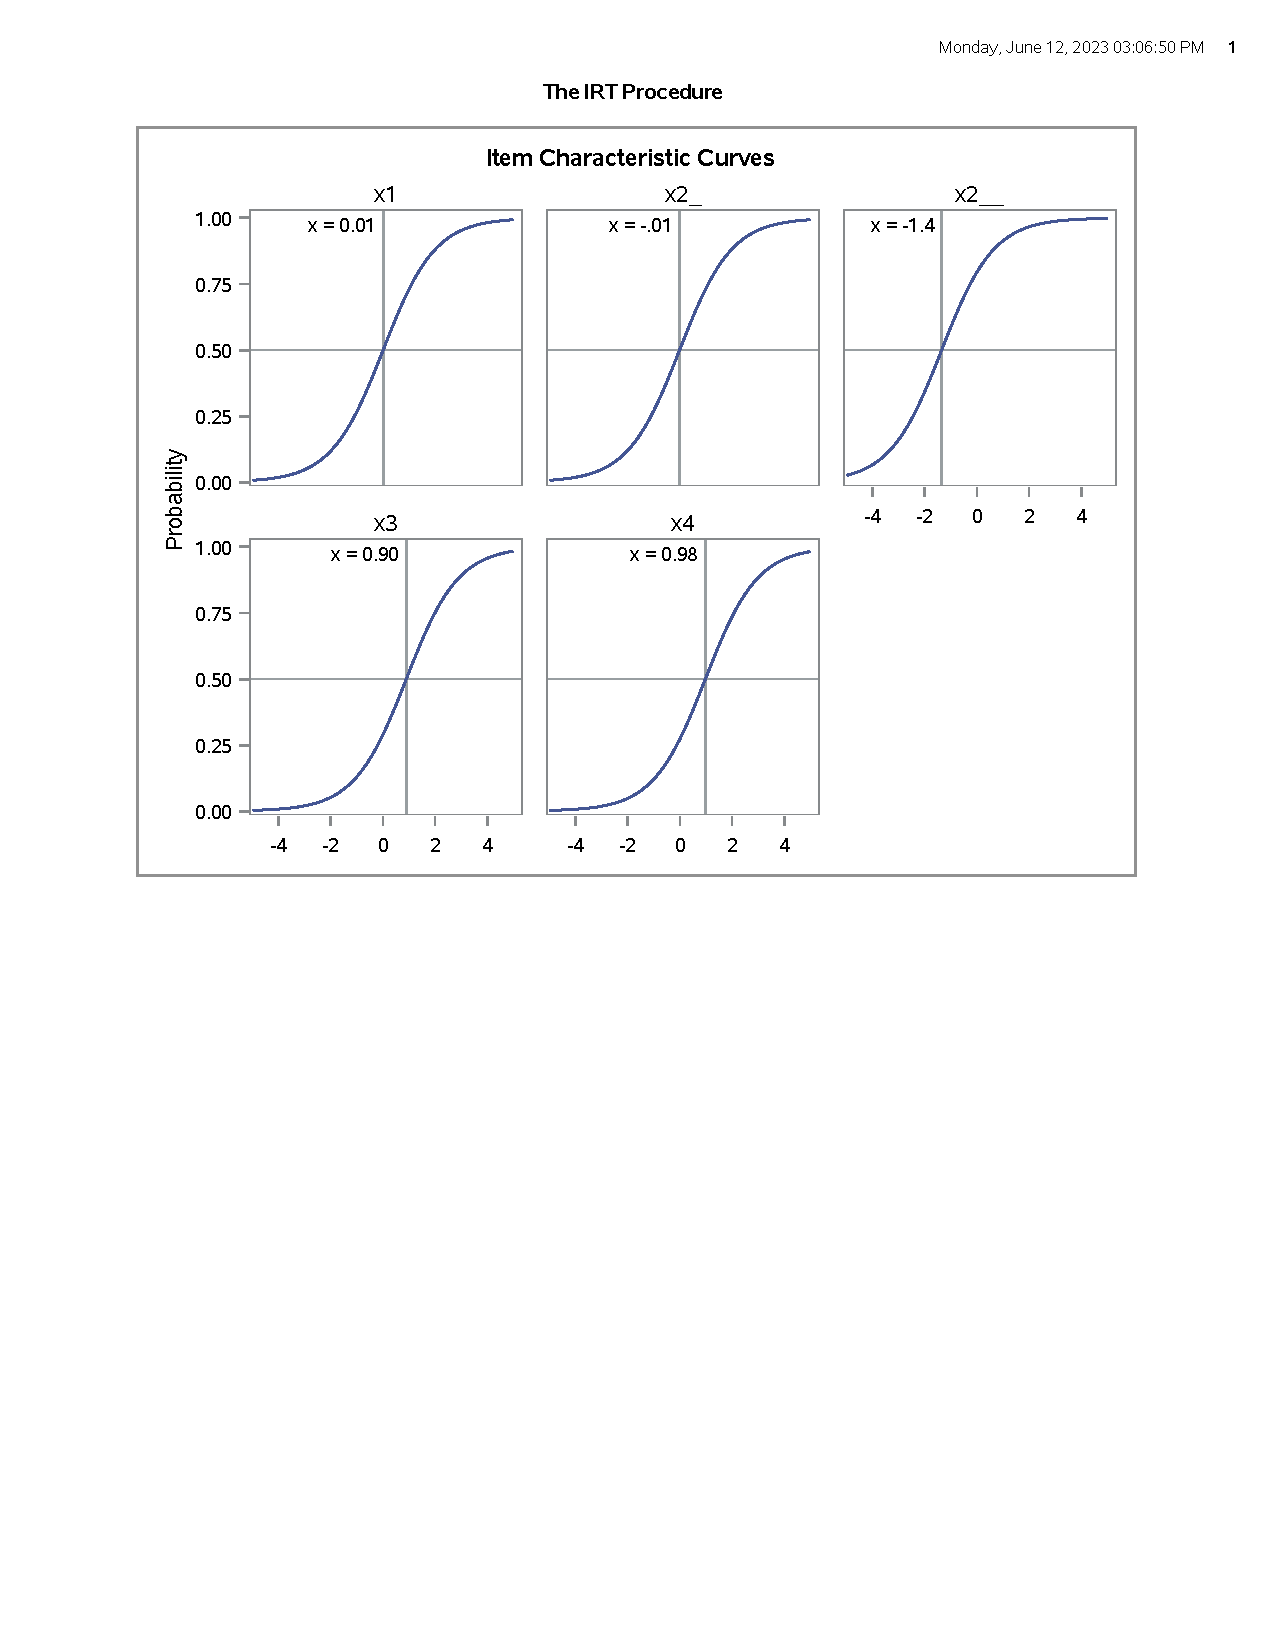
\includegraphics[trim=(2cm 13cm 2cm 2cm), clip, scale=0.5]{icc_split.pdf}
\end{center}
quantification $\beta_{2\_\_}-\beta_{2\_}=1.39$.
\pause
Interpretable for, e.g., educational tests. 
\end{frame}

\begin{frame}{graphical Rasch model}
\begin{block}{graphical Rasch model}
Extension of the Rasch model that incorporates LRD (and DIF) using log linear interaction parameters
\end{block} 
\pause
\begin{center}
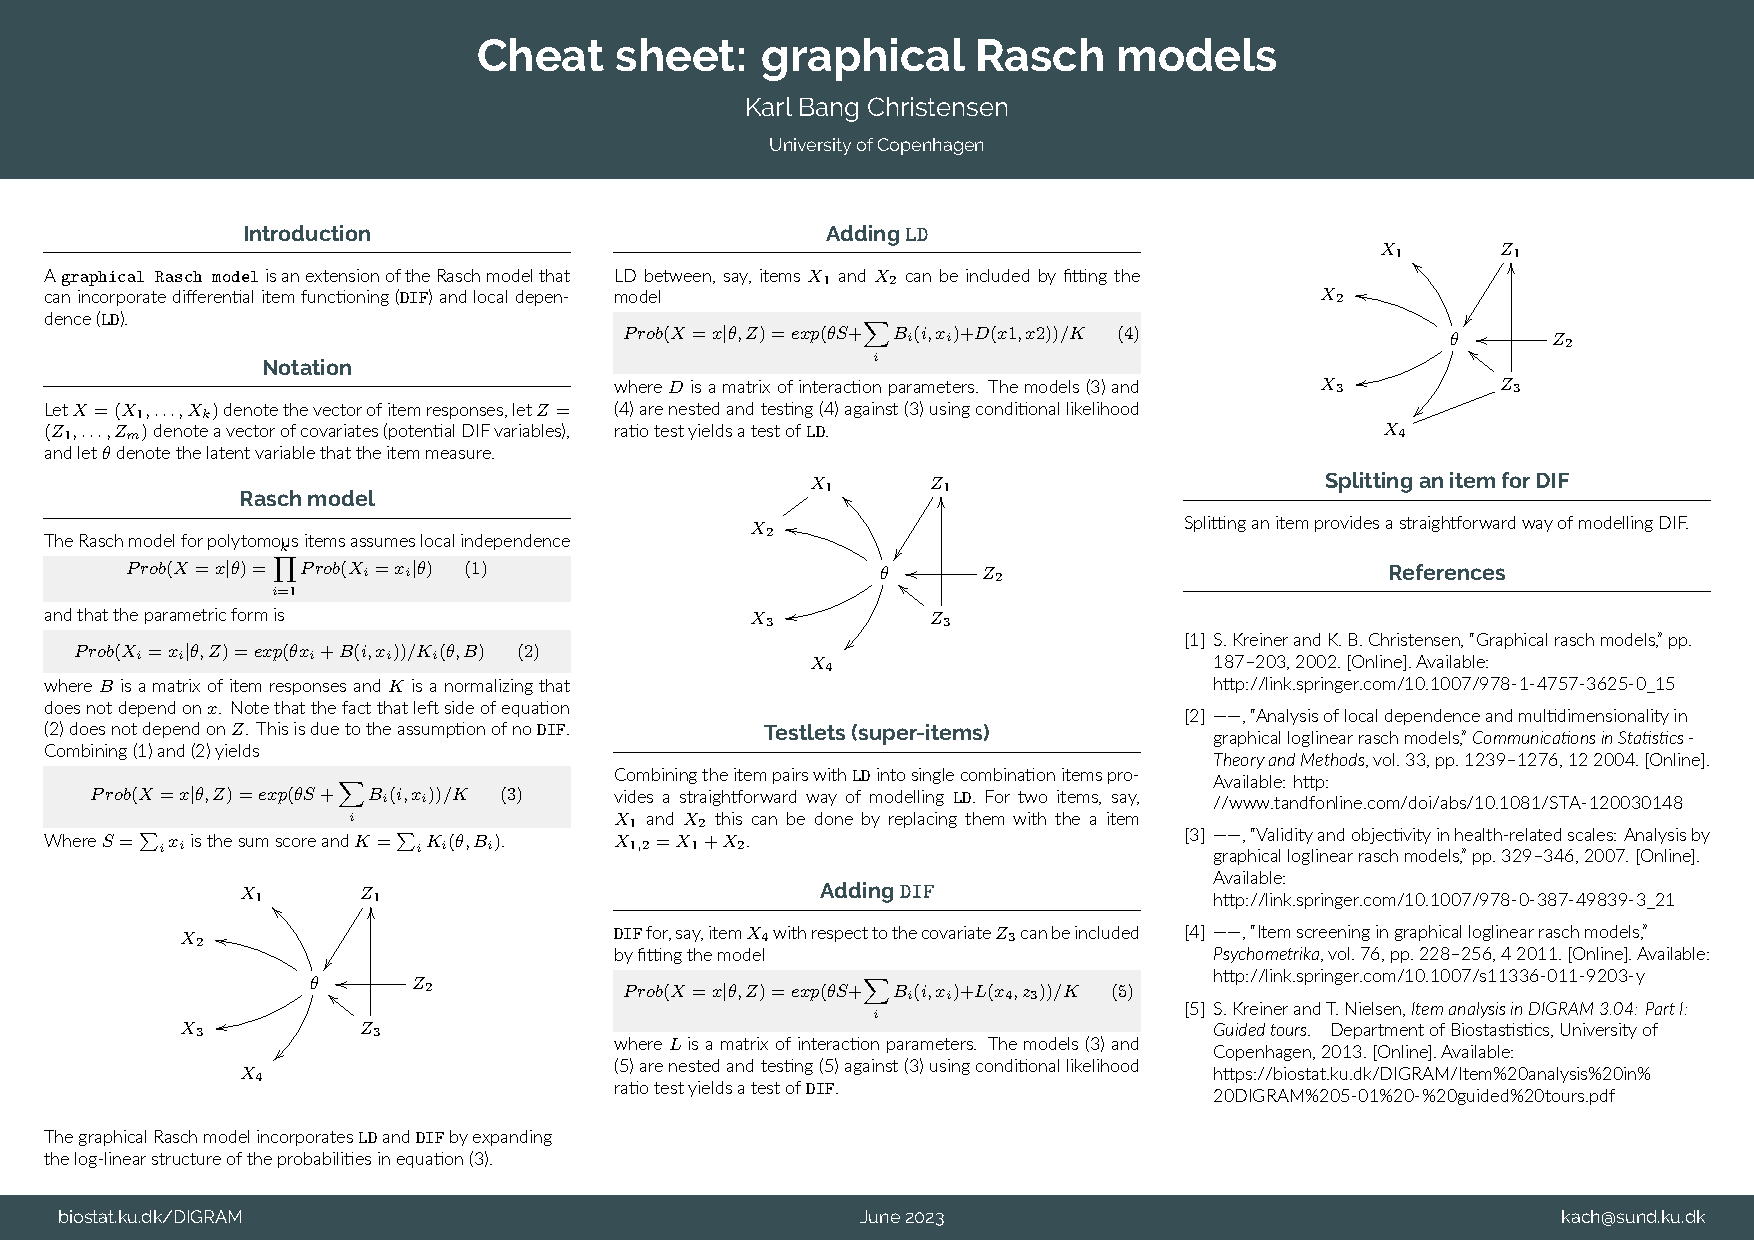
\includegraphics[width=0.45\textwidth]{Cheat_sheet_GRM.pdf}

\includegraphics[scale=0.25]{qrcode_biostat.ku.dk.png}
\end{center}
\url{https://biostat.ku.dk/Rasch/GRM/Cheat_sheet_GRM.pdf}
\end{frame}

\begin{frame}{graphical Rasch model}
Let $I=\{1,\ldots,4\}$ and let, for each $t=0,1,\ldots,4$ 
$$
S(t,I)=\{\mathbf{x}=(x_i)_{i=1,\ldots,4}:\sum_{i=1}^4x_{i}=t\}
$$ 
denote the set of response vectors with sum $t$. Disjoint union
$$
\{0,1\}^k=\bigcup_{t=0}^kS(t,I)
$$
\pause
\begin{block}{Example}
4 items, score $s_v=3$, observed pattern $\boldsymbol{x}_v=(1,1,0,1)$
all possible response patterns with $s_v=3$
$$
\{(1,1,1,0),(1,1,0,1),(1,0,1,1),(0,1,1,1)\}
$$
\end{block}
\end{frame}

\begin{frame}{Data example}
\begin{center}
\begin{tabular}{
>{\columncolor[HTML]{BBBBBB}}c 
>{\columncolor[HTML]{BBBBBB}}c 
>{\columncolor[HTML]{BBBBBB}}c 
>{\columncolor[HTML]{BBBBBB}}c 
>{\columncolor[HTML]{FFFFFF}}r 
>{\columncolor[HTML]{FFFFFF}}r }
\cellcolor[HTML]{34CDF9}x1 & \cellcolor[HTML]{34CDF9}x2 & \cellcolor[HTML]{34CDF9}x3 & \cellcolor[HTML]{34CDF9}x4 & \cellcolor[HTML]{34CDF9}N & \cellcolor[HTML]{34CDF9}\% \\
0 & 0 & 0 & 0 & 17& 23.61 \\
\hline
0 & 0 & 0 & 1 & 2 & 2.78  \\
0 & 0 & 1 & 0 & 3 & 4.17  \\
0 & 1 & 0 & 0 & 4 & 5.56  \\
1 & 0 & 0 & 0 & 4 & 5.56  \\
\hline
0 & 1 & 0 & 1 & 5 & 6.94  \\
1 & 0 & 0 & 1 & 1 & 1.39  \\
0 & 1 & 1 & 0 & 4 & 5.56  \\
1 & 0 & 1 & 0 & 1 & 1.39  \\
1 & 1 & 0 & 0 & 7 & 9.72  \\
\hline
0 & 1 & 1 & 1 & 1 & 1.39  \\
1 & 1 & 0 & 1 & 8 & 11.11 \\
1 & 1 & 1 & 0 & 9 & 12.50 \\
\hline
1 & 1 & 1 & 1 & 6 & 8.33                  
\end{tabular}
\end{center}
\end{frame}

\begin{frame}{graphical Rasch model}
The score distribution 
$$
P(S_v=t|\theta_v=\theta)=
\frac{\exp(t\theta)}{K(\boldsymbol{\beta},\theta)}\gamma(\boldsymbol{\beta};I,t)
$$
is a power series distributions.\footnote{Noack (1950). Annals of Mathematical Statistics, 21, 127-132. \url{www.jstor.org/stable/2236562}} The conditional probability 
$$
P(\boldsymbol{x}_v=\boldsymbol{x}|S_v=t,\theta_v=\theta)=
\frac{\exp(-(x_1\beta_1+x_2\beta_2+x_3\beta_3+x_4\beta_4))}
{\gamma(\boldsymbol{\beta};t,I)}
$$
does not depend on $\theta$. This property is called sufficiency. We can estimate $\boldsymbol{\beta}$ without assumptions about the distribution of $\theta$.\footnote{Andersen (1970). Journal of the Royal Statistical Society B, 32, 283-301.}
\end{frame}

\begin{frame}{Graphical Rasch model}
Extend the conditional probability with an interaction parameter\footnote{Kreiner, Christensen (2002). Statistical Methods for Quality of Life Studies (pp. 187–203). Springer US. \url{https://doi.org/10.1007/978-1-4757-3625-0_15}}

$$
P(\boldsymbol{X}_v=\boldsymbol{x}|S_v=t)=
\frac{\exp(-(x_1\beta_1+..+x_4\beta_4+\delta x_1x_2))}
{\gamma(\boldsymbol{\beta};t,I)}
$$
\pause
\begin{block}{Note}
Equivalent to item splitting (5 parametes).   
\end{block}
\end{frame}


\begin{frame}{Analysis}
\begin{block}{Yens $Q_3$ test statistic}
IRT or Rasch software.
\end{block}
\pause
\begin{block}{Item splitting}
Data manipulation and Rasch software.
\end{block}
\pause
\begin{block}{graphical Rasch model}
Specialized sofware.
\end{block} 
\pause
\begin{block}{simpler analyses..}
..are also feasible.
\end{block} 
\end{frame}


\begin{frame}{simpler analyses}
Consequence of the sufficiency property
\begin{block}{Non-parametric tests of LRD}
Let $R_i=\sum_{j\neq i}X_i$ denote rest-scores. Then for any item pair $(k,k')$
$$
X_k\perp X_{k'}|R_k\;\;\;\;\;\text{and}
\;\;\;\;\;X_i\perp X_{k'}|R_{k'}
$$
\end{block}
old idea\footnote{Tjur (1982). Scandinavian Journal of Statistics, 9, 23-30. \url{http://www.jstor.org/stable/4615850}}
\end{frame}


\begin{frame}{simpler analyses}
\begin{block}{$R_1$}

\includegraphics[width=\textwidth, page=1, clip, trim=0mm 220mm 0mm 10mm]{tjur.pdf}    
\end{block}
\begin{block}{$R_2$}

\includegraphics[width=\textwidth, page=2, clip, trim=0mm 220mm 0mm 10mm]{tjur.pdf}    
\end{block}
\end{frame}

\begin{frame}{Overview}
\begin{itemize}
\item[\checkmark] Small data example four dichotomous items. What is validation ?
\item[\checkmark] Local independence (LI). What does it mean ?
\end{itemize}
\begin{block}{Local response dependence (LRD)}
\begin{itemize}
\item[\checkmark] consequences
\item[\checkmark] analysis
\item[O] interpretation 
\item[O] modelling 
\end{itemize}
\end{block}
\begin{itemize}
\item[O] Data example
\end{itemize}
\end{frame}

\begin{frame}{Interpretation}
\begin{block}{Positive association}
$Q_3$ large, when splitting getting first test item correct makes the second test item easier
\pause
\begin{itemize}
\item (essential) unidimensionality 
\pause
\item items are too similar, redundancy, bifactor model, testlet (super-item) model
\end{itemize}
\end{block}
\begin{block}{Negative association}
$Q_3$ negative, when splitting getting first test item correct makes the second test item more difficult
\pause
\begin{itemize}
    \item multi-dimensionality
\end{itemize}
\end{block}
\end{frame}

\begin{frame}{Overview}
\begin{itemize}
\item[\checkmark] Small data example four dichotomous items. What is validation ?
\item[\checkmark] Local independence (LI). What does it mean ?
\end{itemize}
\begin{block}{Local response dependence (LRD)}
\begin{itemize}
\item[\checkmark] consequences
\item[\checkmark] analysis
\item[\checkmark] interpretation 
\item[O] modelling 
\end{itemize}
\end{block}
\begin{itemize}
\item[O] Data example
\end{itemize}
\end{frame}

\begin{frame}{modelling}
\begin{block}{complicated}
Graphical Rasch model, bifactor IRT model
\end{block}
\pause
\begin{block}{simpler}
Rasch model using teslets (super-items)
\end{block}
\pause
\begin{block}{Complications}
Finding the correct model. Interplay between item fit, DIF and LRD is complicated. Risk of spurious evidence.
\end{block}

\end{frame}


\begin{frame}{Spurious evidence}
\begin{tabular}{ccc}
\xymatrix{
     &X_1\;&                                                               &Y_1\ar[ddl]                  \\
X_2\;&     &                                                               &                             \\
     &     &\ar@/_/[uul]\ar@/_/[ull]\ar@/^/[dll]\ar@/^/[ddl] \;\;\theta\;\;&                  &Y_2\ar[ll]\\
X_3\;&     &                                                               &Y_3\ar[uuu]\ar[ul]           \\
     &X_4\;&                                                               &
}
&&
\begin{tabular}{l}
\\
\\
LI \\
model \\
\\
\\
\end{tabular}
\end{tabular}
\end{frame}

\begin{frame}{Spurious evidence}
\begin{tabular}{ccc}
\xymatrix{
     &X_1\;&                                                               &Y_1\ar[ddl]                  \\
X_2\;\ar@{-}[dd]&     &                                                               &                             \\
     &     &\ar@/_/[uul]\ar@/_/[ull]\ar@/^/[dll]\ar@/^/[ddl] \;\;\theta\;\;&                  &Y_2\ar[ll]\\
X_3\;&     &                                                               &Y_3\ar[uuu]\ar[ul]           \\
     &X_4\;&                                                               &
}
&&
\begin{tabular}{l}
\\
\\
LRD\\ 
model\\
\\
\\
\end{tabular}
\end{tabular}
\end{frame}

\begin{frame}{Spurious evidence}
\begin{tabular}{ccc}
\xymatrix{
     &X_1\;\ar@{-}[rr]&                                                               &Y_1\ar[ddl]                  \\
X_2\;&     &                                                               &                             \\
     &     &\ar@/_/[uul]\ar@/_/[ull]\ar@/^/[dll]\ar@/^/[ddl] \;\;\theta\;\;&                  &Y_2\ar[ll]\\
X_3\;&     &                                                               &Y_3\ar[uuu]\ar[ul]           \\
     &X_4\;&                                                               &
}
&&
\begin{tabular}{l}
\\
\\
DIF \\
model \\
\\
\\
\end{tabular}
\end{tabular}
\end{frame}

\begin{frame}{Spurious evidence}
\begin{tabular}{ccc}
\xymatrix{
     &X_1\;&                                                    &Y_1\ar[ddl]                  \\
X_2\;&     &                                                               &                             \\
     &     &\ar@/_/[uul]\ar@/_/[ull]\ar@/^/[dll]\ar@/^/[ddl] \;\;\theta\;\;&                  &Y_2\ar[ll]\\
X_3\;\ar@{-}[rrr]&     &                                                               &Y_3\ar[uuu]\ar[ul]           \\
     &X_4\;&                                                               &
}
&&True model
\end{tabular}\end{frame}

\begin{frame}{Spurious evidence}
\begin{tabular}{ccc}
\xymatrix{
     &X_1\;&                                                    &Y_1\ar[ddl]                  \\
X_2\;&     &                                                               &                             \\
     &     &\ar@/_/[uul]\ar@/_/[ull]\ar@/^/[dll]\ar@/^/[ddl] \;\;\theta\;\;&                  &Y_2\ar[ll]\\
X_3\;\ar@{-}[rrr]\ar@{-}[rrruuu]&     &                                                               &Y_3\ar[uuu]\ar[ul]           \\
     &X_4\;&                                                               &
}
&&
Spurious evidence
\end{tabular}
\end{frame}

\begin{frame}{Spurious evidence}
\begin{tabular}{ccc}
\xymatrix{
     &X_1\;\ar@{-}[rr]&                                                    &Y_1\ar[ddl]                  \\
X_2\;\ar@{-}[ur]&     &                                                               &                             \\
     &     &\ar@/_/[uul]\ar@/_/[ull]\ar@/^/[dll]\ar@/^/[ddl] \;\;\theta\;\;&                  &Y_2\ar[ll]\\
X_3\;&     &                                                               &Y_3\ar[uuu]\ar[ul]           \\
     &X_4\;&                                                               &
}
&&True model
\end{tabular}
\end{frame}

\begin{frame}{Spurious evidence}
\begin{tabular}{ccc}
\xymatrix{
     &X_1\;\ar@{-}[rr]&                                                    &Y_1\ar[ddl]                  \\
X_2\;\ar@{-}[ur]\ar@{-}[urrr]&     &                                                               &                             \\
     &     &\ar@/_/[uul]\ar@/_/[ull]\ar@/^/[dll]\ar@/^/[ddl] \;\;\theta\;\;&                  &Y_2\ar[ll]\\
X_3\;&     &                                                               &Y_3\ar[uuu]\ar[ul]           \\
     &X_4\;&                                                               &
}
&&
Spurious evidence
\end{tabular}
\end{frame}

\begin{frame}{modelling}

\begin{block}{Spurious evidence}
Is a problem that should also be considered when looking for the correct model. Item screening procedure tries to take this problem into account
\end{block}
General item screening procedure.\footnote{Kreiner, Christensen (2011). Psychometrika, 76, 228–256. \url{https://doi.org/10.1007/s11336-011-9203-y}}


\begin{block}{Multiple testing}
is also a problem and  should also be considered when looking for the correct model.
\end{block}

\begin{block}{Remember}
Can only find sensible model by also looking at item content. Design (e.g. stratified analyses) is a good thing to think about.
\end{block}
\end{frame}

\begin{frame}{Example: Pedi-IKDC}
\begin{block}{evaluates}
anterior cruciate ligament (ACL) deficiency in children, but its construct validity has not been thoroughly assessed.
\end{block} 
\pause
\begin{block}{cohort}
consisting of all children and adolescents in Denmark treated with physeal-sparing ACL reconstruction 2011–2020. Data collected before surgery and at 1 year follow-up.
\end{block}
\end{frame}

\begin{frame}{Example: Pedi-IKDC}

\includegraphics[page=4, trim=60pt 315pt 16pt 10pt, clip, scale=0.35]{Scandinavian_Med_Sci_Sports___2023___Hansen___PediIKDC_exhibits_questionable_measurement_properties_in_a_cohort_of.pdf}

Bifactor model best (not good)\footnote{Hansen et al (2023). Scandinavian Journal of Medicine \& Science in Sports. \url{https://doi.org/10.1111/sms.14413}}
\end{frame}

\begin{frame}{Example: Pedi-IKDC}

\includegraphics[page=5, trim=60pt 120pt 16pt 10pt, clip, scale=0.35]{Scandinavian_Med_Sci_Sports___2023___Hansen___PediIKDC_exhibits_questionable_measurement_properties_in_a_cohort_of.pdf}
\end{frame}

\begin{frame}{Example: HAGOS}
\begin{itemize}
\item The Copenhagen Hip and Groin Outcome Score (HAGOS) questionnaire was developed to obtain a quantitative measure of hip and groin disability in young to middle-aged physically active individuals.
\item N=452 athletes with current groin pain, 18–35 years of age. Danish (N=157, 34.7\%), English (N=146, 32.2\%) or Norwegian (N=149, 33.0\%)  version of HAGOS.
\end{itemize}
\end{frame}

\begin{frame}{Example: HAGOS}
Often evidence of correlated residuals same item pair(s) across language versions.
\begin{center}
\includegraphics[page=3, trim=10pt 10pt 290pt 625pt, clip, scale=0.7]{333full.pdf}
\end{center}
having established reasonable revised scales DIF across language versions could be addressed.
\end{frame}

\begin{frame}{Example: HAGOS}
Symptoms subscale. Item fit

\includegraphics[width=37mm, page=2, clip, trim=20mm 95mm 20mm 10mm]{S_1_fitplot.pdf}
\includegraphics[width=37mm, page=2, clip, trim=20mm 95mm 20mm 10mm]{S_2_fitplot.pdf}
\includegraphics[width=37mm, page=2, clip, trim=20mm 95mm 20mm 10mm]{S_3_fitplot.pdf}

\end{frame}


\begin{frame}{Overview}
\begin{itemize}
\item[\checkmark] Small data example four dichotomous items. What is validation ?
\item[\checkmark] Local independence (LI). What does it mean ?
\end{itemize}
\begin{block}{Local response dependence (LRD)}
\begin{itemize}
\item[\checkmark] consequences
\item[\checkmark] analysis
\item[\checkmark] interpretation 
\item[\checkmark] modelling 
\end{itemize}
\end{block}
\begin{itemize}
\item[O] Data example
\end{itemize}
\end{frame}

\begin{frame}{Data example}
\begin{center}
\begin{tabular}{
>{\columncolor[HTML]{BBBBBB}}c 
>{\columncolor[HTML]{BBBBBB}}c 
>{\columncolor[HTML]{BBBBBB}}c 
>{\columncolor[HTML]{BBBBBB}}c 
>{\columncolor[HTML]{FFFFFF}}r 
>{\columncolor[HTML]{FFFFFF}}r }
\cellcolor[HTML]{34CDF9}x1 & \cellcolor[HTML]{34CDF9}x2 & \cellcolor[HTML]{34CDF9}x3 & \cellcolor[HTML]{34CDF9}x4 & \cellcolor[HTML]{34CDF9}N & \cellcolor[HTML]{34CDF9}\% \\
0 & 0 & 0 & 0 & 17& 23.61 \\
\hline
0 & 0 & 0 & 1 & 2 & 2.78  \\
0 & 0 & 1 & 0 & 3 & 4.17  \\
0 & 1 & 0 & 0 & 4 & 5.56  \\
1 & 0 & 0 & 0 & 4 & 5.56  \\
\hline
0 & 1 & 0 & 1 & 5 & 6.94  \\
1 & 0 & 0 & 1 & 1 & 1.39  \\
0 & 1 & 1 & 0 & 4 & 5.56  \\
1 & 0 & 1 & 0 & 1 & 1.39  \\
1 & 1 & 0 & 0 & 7 & 9.72  \\
\hline
0 & 1 & 1 & 1 & 1 & 1.39  \\
1 & 1 & 0 & 1 & 8 & 11.11 \\
1 & 1 & 1 & 0 & 9 & 12.50 \\
\hline
1 & 1 & 1 & 1 & 6 & 8.33                  
\end{tabular}
\end{center}
\end{frame}

\begin{frame}{Data example}
\begin{itemize}
\item four items (presence of symptom)
\item three person factors (two age groups, gender, four diagnosis group)
\end{itemize}
\begin{block}{Over all model fit}
$z=7.36$, $df=3$, $p=0.0612$    
\end{block}
Conditional likelihood ratio test\footnote{Andersen (1973). Psychometrika, 38, 123–140. \url{https://doi.org/10.1007/BF02291180}}
\end{frame}

\begin{frame}{Data example}
\begin{block}{Item screening..}
..using partial correlation conditioning on rest scores.
\pause
No evidence disclosed.
\pause
No evidence of DIF.
\end{block}
\pause
non parametric tests. Less power then parametric tests (e.g. Rasch model based tests).
\end{frame}

\begin{frame}{Data example}
\begin{block}{LRD}
\begin{tabular}{lrrl}
\hline
Item pair & $\chi^2$ & df & $P$  \\
\hline     
(1,2) & 1.96 & 1 & 0.1611 \\
(1,3) & 0.05 & 1 & 0.8298 \\
(1,4) & 0.19 & 1 & 0.6653 \\
(2,3) & 0.47 & 1 & 0.4931 \\
(2,4) & 1.59 & 1 & 0.2068 \\
(3,4) & 7.12 & 1 & 0.0076\footnote{Also significant after adjustment for multiple testing.} \\
\hline
\end{tabular}
\end{block}
\end{frame}

\begin{frame}{Data example}
\begin{block}{LRD}
$Q_{3,\ast} < 0.2$, but this rule of thumb does not really apply to four items (or to $N=73$).
\end{block}
\pause
Closer inspection shows that the LRD is negative. This is not what $Q_{3,\ast}$ looks for.
\end{frame}

\begin{frame}{Data example}
\begin{block}{DIF}
\begin{tabular}{llrrl}
\hline
Item & person factor & $\chi^2$ & df & $P$  \\
\hline 
1 & age group & 0.03 & 1 & 0.8615 \\
:\\
4 & age group & 0.39 & 1 & 0.5315 \\
\hline 
:\\
\hline 
1 & diagnosis & 0.66 & 3 & 0.8817 \\
2 & diagnosis & 7.62 & 3 & 0.0545 \\
3 & diagnosis &16.92 & 3 & 0.0007\footnote{Also significant after adjustment for multiple testing.} \\
4 & diagnosis & 8.27 & 3 & 0.0407 \\
\hline
\end{tabular}
\end{block}

\end{frame}

\begin{frame}{Data example}
graphical Rasch model
\xymatrix{
     &X_1\;&                                                    &Y_1\ar@{-}[ddd]                  \\
X_2\;&     &                                                               &                             \\
     &     &\ar@/_/[uul]\ar@/_/[ull]\ar@/^/[dll]\ar@/^/[ddl] \;\;\theta\;\;&                  &Y_2\ar@{-}[luu]\ar@{-}[ld]\\
X_3\;\ar@{-}[dr]\ar@{-}[rrr]&     &                                                               &Y_3\ar[ul]           \\
     &X_4\;&                                                               &
}
\end{frame}

\begin{frame}{Data example}
Rasch model
$$
P(\boldsymbol{x}|S=t,\boldsymbol{Z})=
\frac{\exp(-(x_1\beta_1+x_2\beta_2+x_3\beta_3+x_4\beta_4))}
{\gamma(..)}
$$
graphical Rasch model
$$
P(\boldsymbol{x}|S=t,\boldsymbol{Z})=
\frac{\exp\left(-(x_1\beta_1+x_2\beta_2+x_4\beta_4+\delta x_3x_4+x_3\sum_d\beta_3^{(d)}1_{(Z_3=d)})\right)}
{\gamma(\boldsymbol{\beta};t,I)}
$$
this model fits the data. Parameters can be interpreted. Both interactions are significant.


\end{frame}
\end{document}


